\section{Технологический раздел}

В данном разделе будут представлены технические аспекты реализации приложения и демонстрация работы программы.

\subsection{Реализация приложения}

В качестве языка программирования был использован язык Си \cite{clang} по указанию преподавателя. Язык достаточно низкоуровневый и предоставляет полный контроль над сокетами. Большинство функционала пришлось реализовывать вручную.

В качестве среды разработки использовался Visual Studio Code \cite{vscode}.

Был использован объектно ориентированный подход, можно говорить что были выбраны конкретные структуры, описывающие сервер, к ним были написаны функции-методы.

\subsection{Листиги кода}

В листинге \ref{lst:launch} представлена реализация запуска веб-сервера с системным вызовом chroot и деэскалацией привелегий.

\captionsetup{singlelinecheck = false, justification=raggedright}
\begin{lstlisting}[label=lst:launch,caption=Запуск сервера]
int main(int argc, char **argv)
{
  ...
  rlim.rlim_cur = rlim.rlim_max =
      3 + nthreads + nthreads * nslots + 5 * nthreads;

  // need sudo to bind priveledged ports 80, 443
  in_socket = create_socket(srv.host, srv.port);
  if (unblock_socket(in_socket))
    return 1;

  errno = 0;
  // get info about user and group
  if (!user || !(pwd = getpwnam(user)))
    die("getpwnam '%s': %s", user ? user : "null",
        errno ? strerror(errno) : "Entry not found");
  if (!group || !(grp = getgrnam(group)))
    die("getgrnam '%s': %s", group ? group : "null",
        errno ? strerror(errno) : "Entry not found");

  if (chdir(servedir) < 0)
    die("chdir '%s':", servedir);

  // need sudo to chroot
  if (chroot(".") < 0)
    die("chroot");

  // after chroot we cant access
  // /etc/password and get info about
  // user to perform the next step:
  // de-escalation priveledges to regular user

  if (pwd->pw_uid == 0 || grp->gr_gid == 0)
    die("Won't run under root %s for obvious reasons",
        (pwd->pw_uid == 0) ? (grp->gr_gid == 0) ? "user and group" : "user" : "group");

  if (setgroups(1, &(grp->gr_gid)) < 0)
      die("setgroups:");
  if (setgid(grp->gr_gid) < 0)
      die("setgid:");
  if (setuid(pwd->pw_uid) < 0)
  {
      die("setuid:");
  }

  init_thread_pool_for_server(in_socket, nthreads, nslots, &srv);
  return status; // global variable 
}
\end{lstlisting}

На риунке \ref{img:worker} изображена схема алгоритма воркера, который запускается в каждом pthread.

\begin{figure}[H]
    \begin{center}
        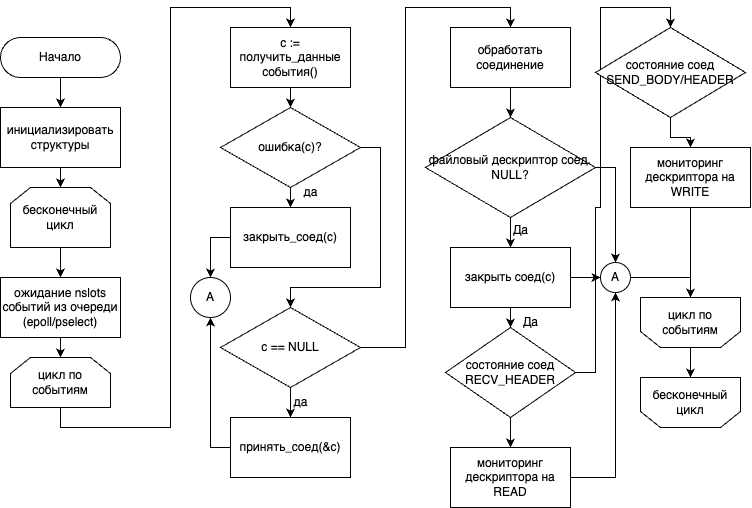
\includegraphics[width=0.95\linewidth]{inc/img/seti_worker.drawio.png}
        \caption{Разработка алгоритма воркера}
        \label{img:worker}
    \end{center}
\end{figure}

Функция обработки соединения включает в себя принятие соединения, поиск подходящего соединения для дропа, принятие заголовка, и парсинг заголовков.

На листинге \ref{lst:get_drop_candidate} представлен поиск соединения для завершения, при новом соединении. Этот алгоритм очень важен для отказоустойчивости при DDOS-атаках, и позволяет выдерживать более 1000 соединений в секунду при использовании select.
Соединение считается приоритетным по:

\begin{enumerate}
    \item состоянию state: VACANT, RECV\_HEADER,
    SEND\_HEADER, SEND\_BODY;
    \item типу ответа: DIRLIST, ERROR, FILE;
    \item прогрессу ответа;
\end{enumerate}

Чем меньше прогресс, тем приоритетнее соединение.

\captionsetup{singlelinecheck = false, justification=raggedright}
\begin{lstlisting}[label=lst:get_drop_candidate,caption=Поиск соединения для отключения]
static struct conn_t * connection_get_drop_candidate(struct conn_t * connection,
  size_t nslots) {
  struct conn_t * c, * minc;
  size_t i, j, maxcnt, cnt;
  for (i = 0, minc = NULL, maxcnt = 0; i < nslots; i++) {
    c = & connection[i];
    for (j = 0, cnt = 0; j < nslots; j++) {
      if (!sockets_same_addr( & connection[i].m_sock_storage, &
          connection[j].m_sock_storage)) {
        continue;
      }
      cnt++;
      if (connection[j].m_state < c -> m_state) {
        c = & connection[j];
      } else if (connection[j].m_state == c -> m_state) {
        if (c -> m_state == CONN_SEND_BODY &&
          connection[i].m_resp.m_type != c -> m_resp.m_type) {
          if (connection[i].m_resp.m_type < c -> m_resp.m_type) {
            c = & connection[j];
          }
        } else if (connection[j].m_progress < c -> m_progress) {
          c = & connection[j];
        }
      }
    }
    if (cnt > maxcnt) {
      minc = c;
      maxcnt = cnt;
    }
  }

  return minc;
}
\end{lstlisting}

На листинге \ref{lst:conn} отображена функция, отвечающая за установку соединения.

\captionsetup{singlelinecheck = false, justification=raggedright}
\begin{lstlisting}[label=lst:conn,caption=Установка соединение]
struct conn_t * accept_con(int in_socket, struct conn_t * connection,
  size_t nslots) {
  struct conn_t * c = NULL;
  size_t i;
  for (i = 0; i < nslots; i++) {
    if (connection[i].m_file_descriptor == 0) {
      c = & connection[i];
      break;
    }
  }
  if (i == nslots) {
    c = connection_get_drop_candidate(connection, nslots);
    if (c == NULL)
      return NULL;
    c -> m_resp.m_status = 0;
    log_con(c);
    reset_con(c);
  }
  if ((c -> m_file_descriptor =
      accept(in_socket, (struct sockaddr * ) & c -> m_sock_storage, &
        (socklen_t) {
          sizeof(c -> m_sock_storage)
        })) < 0) {
    if (errno != EAGAIN && errno != EWOULDBLOCK) {
      log_warn("accept:");
    }
    return NULL;
  }
  if (unblock_socket(c -> m_file_descriptor)) {
    return NULL;
  }
  return c;
}
\end{lstlisting}

\subsection{Демонстрация работа программы}

Для демонстрации корректности работы прогаммы был написан простой веб-сайт, состоящий из трех файлов: index.html, styles.css, interaction.js. На рисунке \ref{img:work1} показан веб-сайт открытый в браузере Firefox. Стили работают корректно, при нажатии на фотографию котенка выводится alert.

\begin{figure}[H]
    \begin{center}
        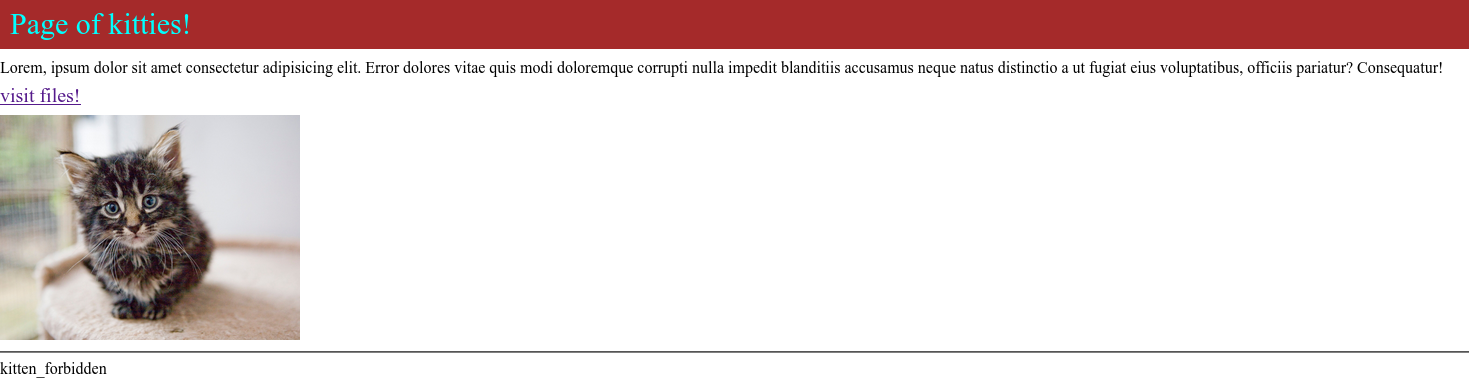
\includegraphics[width=0.95\linewidth]{inc/img/work1.png}
        \caption{Демонстрация работы программы на index.html}
        \label{img:work1}
    \end{center}
\end{figure}

На рисунке \ref{img:work2} показана работа списков файлов в директории. Вложенные директории, ссылки, файлы на русском языке работают корректно.

\begin{figure}[H]
    \begin{center}
        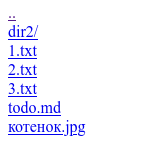
\includegraphics[width=0.25\linewidth]{inc/img/work2.png}
        \caption{Демонстрация работы программы со списком файлов}
        \label{img:work2}
    \end{center}
\end{figure}

Для демоснтрации работы сервера на больших файлах был использован образ установки ArchLinux, весящий 800 Мб, команда wget и сравнение хешей файлов с помощью программы md5sum.

\begin{figure}[H]
    \begin{center}
        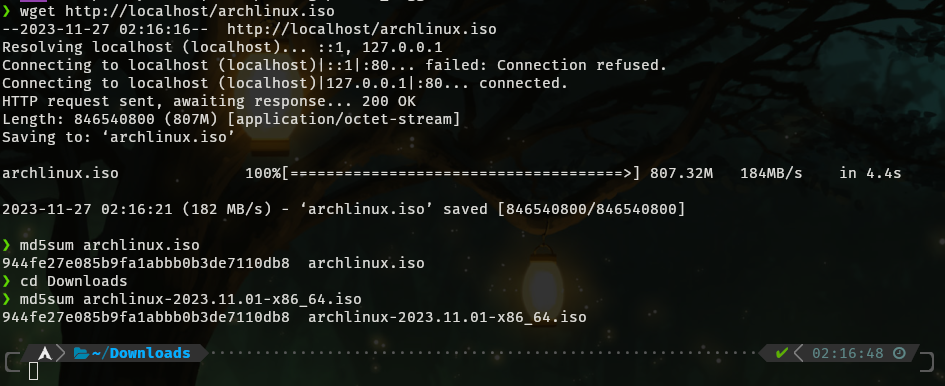
\includegraphics[width=0.95\linewidth]{inc/img/mdsum.png}
        \caption{Демонстрация работы программы на большом файле}
        \label{img:work1}
    \end{center}
\end{figure}


\subsection{Вывод}

Программа была реализована на языке Си, проведена проверка на корректость, пройденная успешно.